\documentclass[11pt,spanish,a4paper]{article}
% Versión 1.er cuat 2021 Víctor Bettachini < bettachini@df.uba.ar >

% Versión 1.er cuat 2021 Víctor Bettachini < bettachini@df.uba.ar >

\usepackage[T1]{fontenc}
\usepackage[utf8]{inputenc}

\usepackage[spanish, es-tabla]{babel}
\def\spanishoptions{argentina} % Was macht dass?
% \usepackage{babelbib}
% \selectbiblanguage{spanish}
% \addto\shorthandsspanish{\spanishdeactivate{~<>}}

\usepackage{graphicx}
\graphicspath{{./figuras/}}
% \usepackage{float}

\usepackage[arrowdel]{physics}
\newcommand{\pvec}[1]{\vec{#1}\mkern2mu\vphantom{#1}}
% \usepackage{units}
\usepackage[separate-uncertainty=true, multi-part-units=single, locale=FR]{siunitx}
\usepackage{isotope} % $\isotope[A][Z]{X}\to\isotope[A-4][Z-2]{Y}+\isotope[4][2]{\alpha}

\usepackage{tasks}
\usepackage[inline]{enumitem}
% \usepackage{enumerate}

\usepackage{hyperref}

% \usepackage{amsmath}
% \usepackage{amstext}
\usepackage{amssymb}

\usepackage{tikz}
\usepackage{tikz-dimline}
\usetikzlibrary{math}
\usetikzlibrary{arrows.meta}
% \usetikzlibrary{snakes}
% \usetikzlibrary{calc}
\usetikzlibrary{decorations.pathmorphing}
\usetikzlibrary{patterns}

\usepackage[hmargin=1cm,vmargin=1.6cm,nohead]{geometry}
% \voffset-3.5cm
% \hoffset-3cm
% \setlength{\textwidth}{17.5cm}
% \setlength{\textheight}{27cm}

\usepackage{lastpage}
\usepackage{fancyhdr}
\pagestyle{fancyplain}
\fancyhead{}
\fancyfoot{{\tiny \textcopyright DF, FCEyN, UBA}}
\fancyfoot[C]{ {\tiny Actualizado al \today} }
\fancyfoot[RO, LE]{Pág. \thepage/\pageref{LastPage}}
\renewcommand{\headrulewidth}{0pt}
\renewcommand{\footrulewidth}{0pt}


\begin{document}
\begin{center}
	\textbf{Física 2} (Físicos) \hfill \textcopyright {\tt DF, FCEyN, UBA}\\
	\textsc{\LARGE Interferencia por división de frente de onda}
\end{center}

Los ejercicios con (*) entrañan una dificultad adicional. Son para investigar después de resolver los demás.


\begin{enumerate}

\subsection*{Lámina de caras paralelas}

\item En una lámina de caras paralelas indique la zona del espacio en que se observa interferencia para fuente puntual y para fuente extensa.
En el primer caso calcule la posición de las imágenes de la fuente. 


\item
\begin{minipage}[t][2.2cm]{0.6\textwidth}
En la lámina de caras paralelas que se indica en la figura, indique qué condición debe cumplirse para que los rayos 1 y 2 interfieran constructivamente.
Cuando eso sucede, ¿qué pasa con los rayos 3 y 4?
¿Qué sucede si se usan otras relaciones entre los índices? ($n_{1}>n_{2}>n_{3}$).
\end{minipage}
\begin{minipage}[c][1cm][t]{0.35\textwidth}
	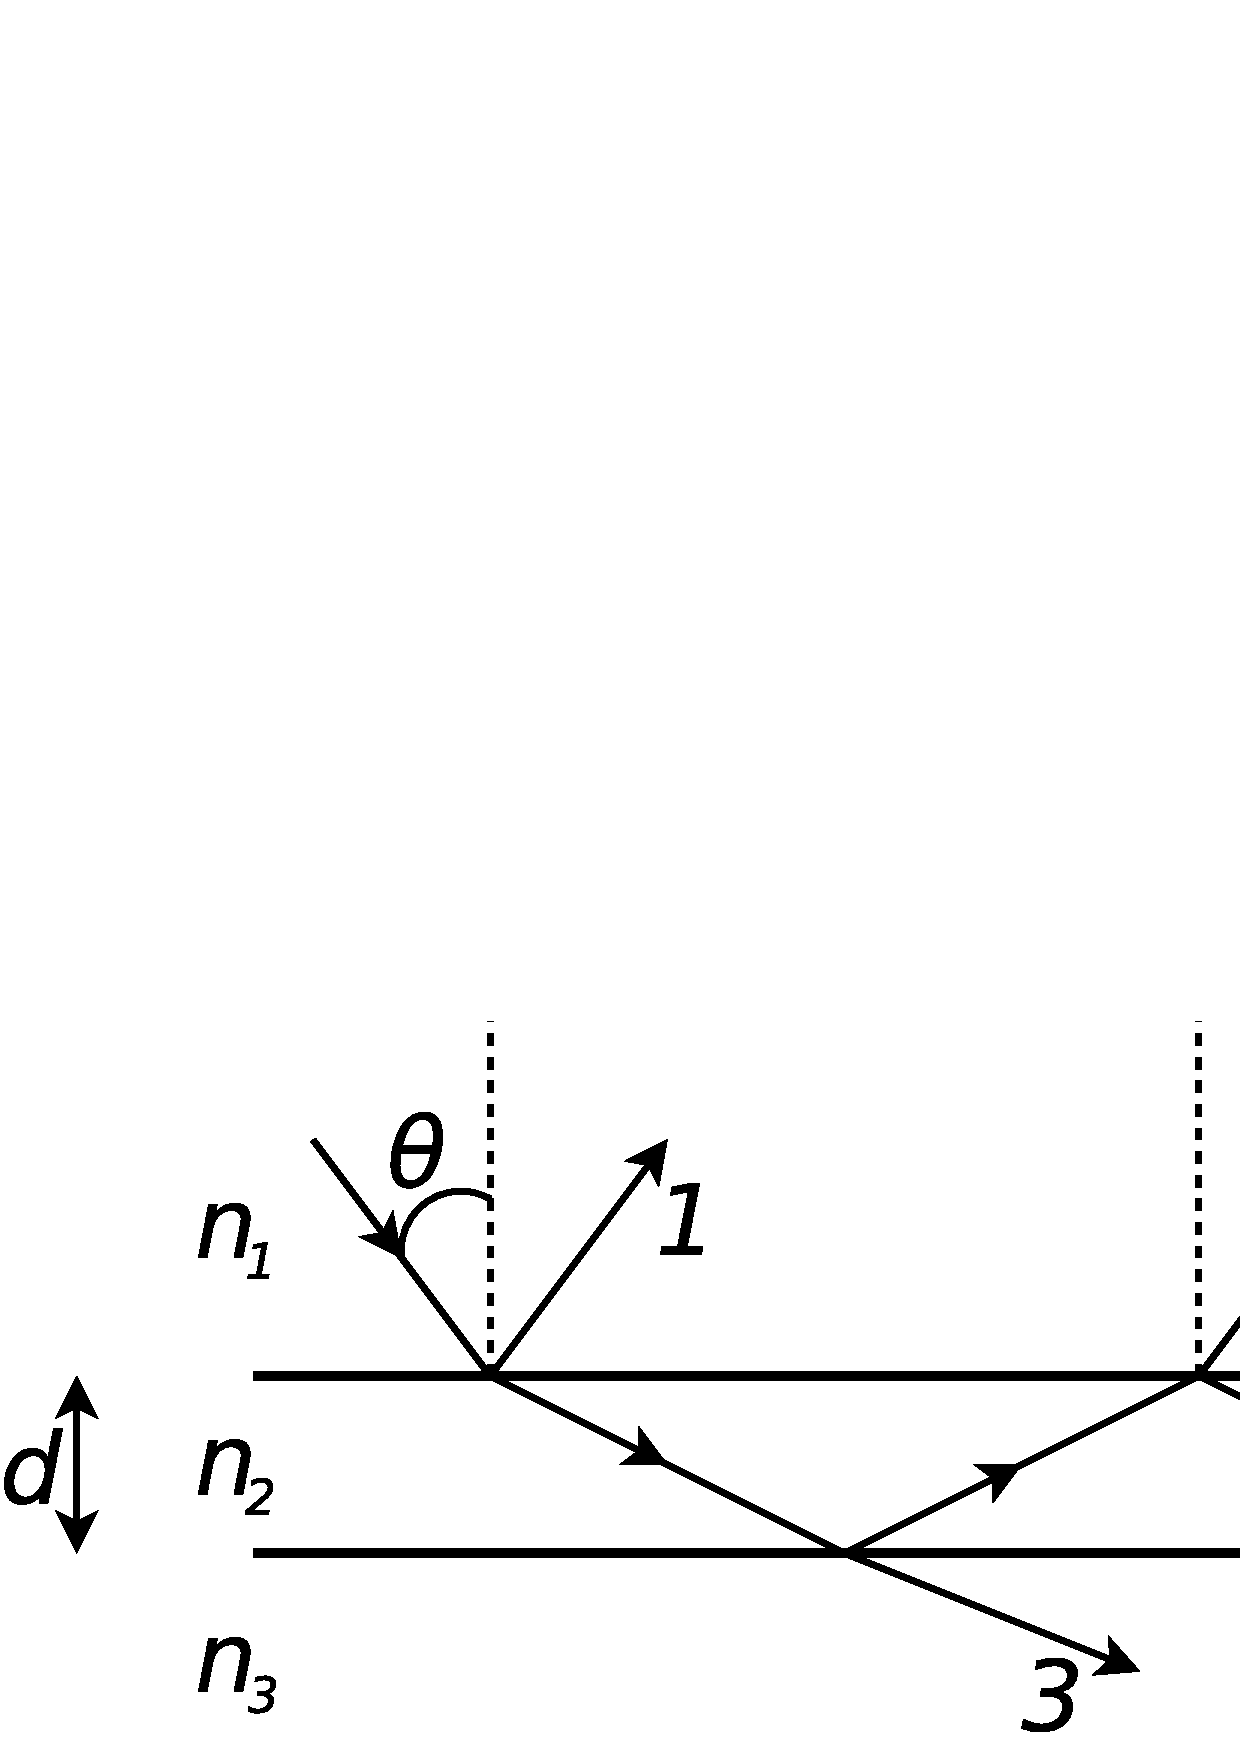
\includegraphics[width=\textwidth]{ej5-21}
\end{minipage}


\item Una lámina de vidrio de \SI{0.40}{\micro\metre} de espesor es iluminada por un haz de luz blanca normal a la lámina.
El índice de refracción es de \num{1.5}.
¿Qué longitudes de onda del espectro visible, \SIrange{400}{790}{\nano\metre}, serán intensificadas en el haz reflejado?



\item ¿Por qué se llaman franjas de igual inclinación a las que aparecen en una lámina de caras paralelas iluminada por una fuente extensa? 

\section*{Cuñas - Anillos de Newton}

\item Una cuña de aire es iluminada de tal forma que si incide luz de longitud de onda \(\lambda = \SI{5000}{\angstrom}\) normalmente a la cara inferior, produce
franjas paralelas cuya distancia entre mínimos es \SI{1}{\milli\metre}.
Describir la cuña. 


\item Se observan anillos de Newton por reflexión, iluminándose una lente plano--convexa con luz de longitud de onda \(\lambda = \SI{650}{\nano\metre}\).
¿Qué radio de curvatura tiene la lente si el segundo anillo oscuro tiene \(d = \SI{2.6}{\milli\metre}\) de diámetro? 



\item
\begin{minipage}[t][4.3cm]{0.7\textwidth}
Se observan anillos de Newton mediante una lámina de vidrio de índice de refracción $n_3$, una lente de vidrio con $n_1 \ne n_3$ y un líquido de $n_2$ intermedio entre $n_1$ y $n_3$ (ver figura). 
\begin{enumerate}
\item ¿Son oscuros o brillantes los centros del sistema de anillos observados respectivamente por reflexión y transmisión? 
\item Suponga ahora que el líquido tiene un índice $n_2 = \num{1.59}$.
Si se observan los anillos por reflexión siendo $\lambda = \SI{5900}{\angstrom}$, y el radio del quinto anillo es de \SI{2}{\milli\metre}, ¿cuál es el radio de curvatura
de la lente?
\end{enumerate}
\end{minipage}
\begin{minipage}[c][0cm][t]{0.25\textwidth}
	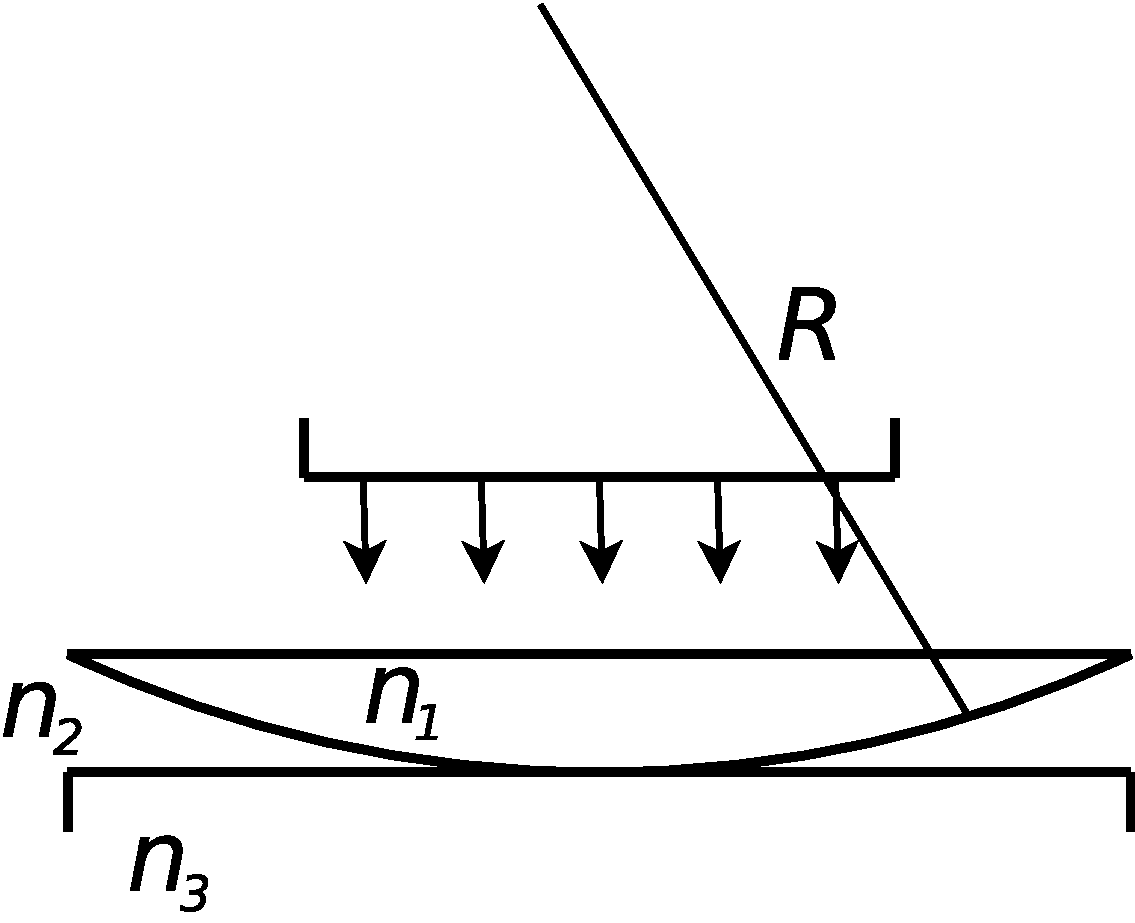
\includegraphics[width=\textwidth]{ej5-26}
\end{minipage}



\item Se observan anillos de Newton con una lente plano--convexa situada sobre un vidrio plano, con aire entre medio.
¿Qué pasa con la diferencia entre los cuadrados de dos radios consecutivos si: 
\begin{enumerate}
	\item Se cambia la lente por otra también plano-convexa del mismo radio de curvatura, pero de mayor índice de refracción? 
	\item Se coloca agua en vez de aire entre la lente y la lámina de vidrio? 
\end{enumerate}



\item Con el mismo dispositivo de los problemas anteriores se observan anillos de Newton por reflexión.
¿Es oscuro o claro el centro de la figura de interferencia?
¿Cuál es el radio del tercer anillo brillante?
¿Qué sucede con los anillos para un ligerísimo desplazamiento hacia arriba de la lente: convergen hacia el centro o se alejan de éste?
¿Por qué? 
Datos: $R = \SI{1}{\metre}$; $d = \SI{0.013}{\milli\metre}$; $\lambda = \SI{5000}{\angstrom}$; $n_1 = \num{1.5}$; $n_2 = \num{1.3}$; $n_3 = \num{1.4}$.



\item En un dispositivo para observar anillos de Newton el espacio entre la lente y la lámina de vidrio está lleno de líquido.
Se observan anillos por transmisión.
La longitud de onda empleada es $\lambda = \SI{5890}{\angstrom}$ y el radio de curvatura de la lente es de \SI{10}{\metre}.
Hallar el índice de refracción del líquido sabiendo que el radio del tercer anillo brillante es de \SI{3.65}{\milli\metre}.



\item
\begin{minipage}[t][0cm]{0.7\textwidth}
Considere el dispositivo de anillos de Newton modificado que se muestra en la figura.
Se observan anillos por reflexión. 
\end{minipage}
\begin{minipage}[c][1.5cm][t]{0.25\textwidth}
	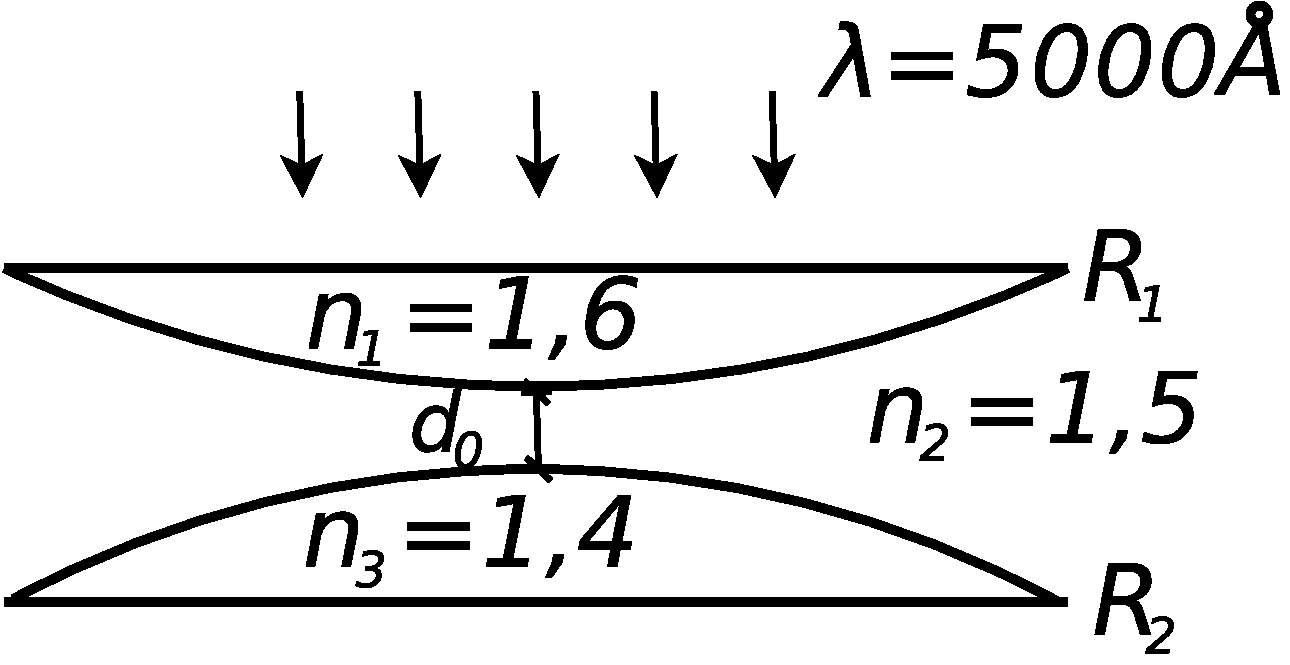
\includegraphics[width=\textwidth]{ej5-30}
\end{minipage}
\begin{enumerate}
	\item ¿Para qué valores de $d_0$ el centro de los anillos corresponde a un máximo? 
	\item Hallar el mínimo valor de $d_0$ para el cual el centro de los anillos corresponde a un mínimo. 
	\item Con el valor de $d_0$ hallado en b), calcular la relación que debe existir entre los radios de las lentes, $R_2 = R_2(R_1)$, para que el radio del primer anillo oscuro verifique $r_1^2 = \SI{e+15}{\angstrom\squared}$
\end{enumerate}

\input{frenteVSAmplitud}


\end{enumerate}

\end{document}
